\section{Target Platform}
In this learning project we are developing applications, for children with autism, using the android platform. The android platform was chosen because this project is part of a multi project, which began the development of the Giraf system.\cite{SW6Android2012}\\
---The initial decision decision to work with the android platform seems to be based on the availability of mobile devices to the students.\cite{adminreport}
However, with the budget supplied by AAU, we had the opportunity to exchange the hardware used in the 2011 6'th semester reports, however this has not included smart phones.\\
In selecting a new tablet we had to make considerations:
\begin{itemize}
	\item Popularity of the tablet type can help in distributing the system. Both among early adapters and potential customers.
	\item Accessibility of the OS is a big factor, whether or not we can construct a system on it.
	\item Design and Variety of the physical tablet can figure in.
\end{itemize}
As seen in figure\ref{fig:QuarterlySales}, the two leading operating systems for mobile devices are Apple's iOS and Google's Android.
Being the more widespread of the two, Apple's iOS tablet, the iPad could have been a viable candidate to replace android tablets based entirely on popularity.\\
However, there are some limitations when developing for iOS.
For one, the iOS Development Environment Xcode currently only runs on Macintosh computers, compared to Android that can use the more universal Eclipse environment.\cite{developApple}\cite{androidDevelopers}\\
There are also only 3 variants of the iPad, where two are earlier variants of the latest design, as apple has a monopoly on developing for iOS.
Android Tablets are far more diverse, having many different manufacturers such as HTC\cite{htcflyer}, Samsung\cite{galaxytabs} and Medion.\cite{mediontablet}
The more variety in manufacturers, will allow us to shop around for the best possible fit.\\
All this is overshadowed by that transforming the system into iOS would most likely leave very little time to create new features.\\

We decided to stay with android, but to  upgrade to version 3.2\cite{android32}. 
This version has been chosen because, it is the first version developed mainly for tablets, and it is going to be supported for the duration of the project.
So ordering several Samsung Galaxy Tablets 10.1, based on its larger screen, the android 3.2 OS and the apparent good results the last semester group had with the older Samsung Tablets.---

\begin{figure}
	\centering
		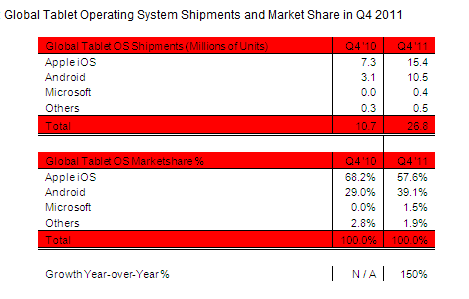
\includegraphics{images/QuarterlySales.png}
	\caption{Shipments refer to sell-in. Numbers are rounded. The definition of tablet does not include e-book readers.\cite{strategyanalytics}}
	\label{fig:QuarterlySales}
\end{figure}



Android is an open-source platform developed for mobile devices. The Android Open Source Project(AOSP) is maintained and further developed by the Open Handset Alliance(OHA), which is led by Google \cite{androidPhilosophy}. The companies from the OHA contributes to the project, these contributions are often made in form of engineering resources.

Android has a large community, spread over various websites, with different areas of expertise. This provides developers of android applications, with a community where they can find help with their nich� \cite{androidCommunity}.
Google, which is head of the android development, also has a website for teaching application developers how to program for the android platform \cite{androidDevelopers}. On Google�s website they also provide various tutorials, so one can easily get started developing for the android platform.

In this project we have been provided with several Samsung Galaxy Tablets 10.1 
\cite{tablet}. The firmware on the tablets is version 3.2\\

NOTE: Stod der ikke noget andet her? Jeg kan ikke finde det mere.